% !TEX encoding = UTF-8 Unicode
%%%%%%%%%%%%%%%%%%%%%%%%%%%%%%%%%%%%%%%%%%%%%%%%%%%%%%%%%%%%%%%%%%%%
%
% Tampereen yliopisto
% Luonnontieteiden tiedekunta
% Matematiikka
%
% Kandidaattitutkielman malli.
% Tutkielman matemaattinen sisältö on prof. Seppo Hyyrön.
%
% Päivitetty 23.9.2018
%
%%%%%%%%%%%%%%%%%%%%%%%%%%%%%%%%%%%%%%%%%%%%%%%%%%%%%%%%%%%%%%%%%%%%
% Yli 60-sivuiset pro gradu -tutkielmat painetaan kaksipuolisina. Jos pro gradu -tutkielmassa on korkeintaan 60 sivua, se painetaan yksipuolisena eli vain paperin yhdelle puolelle. Näin sen vuoksi, että kovin ohuen tutkielman selkään ei mahdu tekijän nimeä. Sivumäärään lasketaan tutkielman kaikki sivut nimiösivusta viimeiseen liitesivuun asti.
\documentclass[a4paper,12pt,leqno,oneside]{report} % jos korkeintaan 60 sivua
%\documentclass[a4paper,12pt,leqno,twoside]{report} % jos yli 60 sivua
\usepackage[utf8]{inputenc}
\usepackage[T1]{fontenc}
\usepackage[finnish]{babel}
\usepackage[intlimits]{amsmath}
%\usepackage{amssymb} % Ei tarvita, kun käytetään makropakettia newtxmath.
\usepackage{amsthm}
\usepackage{booktabs}

% Fontteina Times ja Helvetica.
\usepackage[scale=0.94]{tgheros} % Helvetica tekstifontit.
\usepackage{newtxtext} % Times tekstifontit.
\usepackage[vvarbb]{newtxmath} % Times matematiikkafontit.

% Vaihtoehtoisesti fontteina voi käyttää LaTeXin oletusarvoista Computer Modern -kirjainperhettä (poista tällöin edelliset komennot).
%\usepackage{lmodern}

\usepackage{bm} % Matematiikkatilan lihavat kursiivikirjaimet.
\usepackage{enumerate} % Luetelmanumeroiden muokkaamiseen.
%\usepackage{pdfpages} % Pdf-muotoisten liitteiden liittämiseen.

% Väliotsikoiden tyyliä muokataan makropaketilla titlesec. Jos tarvitset otsikkotasoa \subsubsection, niin muuta optio small muotoon medium.
\usepackage[rm,bf,small,pagestyles]{titlesec}
\titleformat{\chapter}{\normalfont\rmfamily\bfseries\LARGE}{\thechapter}{1em}{}
\titlespacing*{\chapter}{0pt}{-25pt}{30pt}

% Ulkoiset kuvatiedostot liitetään makropaketin graphicx komennolla \includegraphics.
\usepackage{graphicx}
\graphicspath{{Kuvat/}} % Ulkoisten kuvatiedostojen kansio.

% Kelluvien kuvien ja taulukoiden oletusarvoista sijoittelua voi säätää makropaketin float komennolla \floatplacement.
\usepackage{float}
\floatplacement{figure}{htb}	% oletusarvo on tbp
\floatplacement{table}{htb}		% oletusarvo on tbp

% Kuvien ja taulukoiden otsikot muotoillaan makropaketilla caption.
\usepackage[%
margin=\leftmargini,
labelfont=bf,
labelsep=period,
tableposition=top,
]{caption}

% Hypertekstilinkkejä ja url-osoitteita voi tehdä makropaketilla hyperref, jota on kutsuttava viimeiseksi. Optioilla pdftitle ja pdfauthor pdf-tiedostoon lisätään tutkielman ja tekijän nimet metatietoina.
\usepackage[%
pdftitle={Algebrallista koodausteoriaa},
pdfauthor={Eemeli Lottonen},
hidelinks,
pdfpagemode=UseNone,
pdfstartview=FitH]{hyperref}
% Verkko-osoitteet tulostetaan samalla fontilla kuin muukin teksti:
\urlstyle{same}

% Kasvatetaan palstan korkeutta neljä riviä:
\addtolength{\textheight}{4\baselineskip}
\addtolength{\topmargin}{-3.5\baselineskip}

\setlength{\textwidth}{401pt} % Palstan leveys.
\setlength{\footskip}{4\baselineskip} % Sivunumeron etäisyys palstan alareunasta.

% Asetetaan marginaalit yhtäsuuriksi:
\setlength{\oddsidemargin}{0.5\paperwidth}
\addtolength{\oddsidemargin}{-0.5\textwidth}
\addtolength{\oddsidemargin}{-1in}
\setlength{\evensidemargin}{\oddsidemargin}

% Kandidaattitutkielmassa tarvitaan harvennettua riviväliä, jotta korjausmerkinnöille jää tilaa. Gradussa riviväliä ei harvenneta, joten seuraava rivi jätetään silloin pois.
\linespread{1.35}\selectfont % vain kandidaattitutkielmassa

% Lauseiden teksti kursivoidaan:
\theoremstyle{plain}
\newtheorem{lause}{Lause}[chapter]

% ApuLauseiden teksti kursivoidaan:
\theoremstyle{plain}
\newtheorem{apulause}[lause]{Apulause}

% Määritelmien ja esimerkkien tekstiä ei yleensä kursivoida.
\theoremstyle{definition}
\newtheorem{maaritelma}{Määritelmä}[chapter]
\newtheorem{esimerkki}{Esimerkki}[chapter]

\DeclareMathOperator{\wt}{wt}
\DeclareMathOperator{\im}{Im}

% Huomautuksia ei numeroida:
\theoremstyle{remark}
\newtheorem*{huomautus}{Huomautus}

% Kaavat numeroidaan luvuittain:
\numberwithin{equation}{chapter}

% Pitkä yhtälöketju voidaan jakaa eri sivuille:
\allowdisplaybreaks[1]

% Muutetaan lähdeluettelon otsikko, joka on oletusarvoisesti "Kirjallisuutta".
\AtBeginDocument{\renewcommand*{\bibname}{Lähteet}}


% 1 x n matriisit paremmiksi
\renewcommand\arraystretch{0.8}
% isoille matriiseille
\newenvironment{bbmatrix}{
    \renewcommand{\arraystretch}{1.2}
    \begin{bmatrix}
}
{\end{bmatrix}\renewcommand{\arraystretch}{0.8}}
% Komento \Kuukausi tulostaa nykyisen kuukauden nimen isolla alkukirjaimella kirjoitettuna.
% \newcommand*{\Kuukausi}{\ifcase\ \month\ \or\ Tammi\or\ Helmi\or\ Maalis\or\ Huhti\or\ Touko\or\ Kesä\or\ Heinä\or\ Elo\or\ Syys\or\ Loka\or\ Marras\or\ Joulu\fi kuu}
\newcommand*{\Kuukausi}{\ifcase\month\or{}Tammi\or{}Helmi\or{}Maalis\or{}Huhti\or{}Touko\or{}Kesä\or{}Heinä\or{}Elo\or{}Syys\or{}Loka\or{}Marras\or{}Joulu\fi kuu}

    % Joitain komentoja matemaattisia merkintöjä varten:
    \newcommand*{\Nset}{\mathbb{N}}  % luonnollisten lukujen joukko
    \newcommand*{\Zset}{\mathbb{Z}}  % kokonaislukujen joukko
    \newcommand*{\Qset}{\mathbb{Q}}  % rationaalilukujen joukko
    \newcommand*{\Rset}{\mathbb{R}}  % reaalilukujen joukko
    \newcommand*{\Cset}{\mathbb{C}}  % kompleksilukujen joukko

    % Makropaketin amsmath käyttöohjeissa (amsldoc.pdf s. 18--19) suositellaan itseisarvolle ja normille seuraavia komentoja:
    \newcommand*{\abs}[1]{\left\lvert#1\right\rvert}   % itseisarvo
    \newcommand*{\norm}[1]{\left\lVert#1\right\rVert}  % normi

    % Matriiseille ja vektoreille kannattaa määritellä oma komentonsa. Komennon \bm asemesta voi tässä käyttää komentoa \mathbf, jos halutaan käyttää pystyjä eikä kursivoituja kirjaimia.
    \newcommand*{\mx}{\bm}  % matriisi tai vektori

    % Suomessa käytettävä integraaliinsijoitusmerkki saadaan alla olevalla komennolla \sijoitus{alaraja}{yläraja}. Tämän kanssa on hyvä käyttää amsmath-makropaketin optiota [intlimits], jolla integrointirajat asetetaan integraalimerkin ylä- ja alapuolelle eikä viereen kuten LaTeXissa oletusarvoisesti.
    \makeatletter
    \@ifpackageloaded{newtxmath}
    {\newcommand*{\sijoitus}[2]{\mathop{\bigg/}\limits_{\mspace{-11mu}#1}^{\mspace{10mu}#2}}}
    {\newcommand*{\sijoitus}[2]{\mathop{\Big/}\limits_{\mspace{-19mu}#1}^{\mspace{19mu}#2}}}
    \makeatother

    %%%%%%%%%%%%%%%%%%%%%%%%%%%%%%%%%%%%%%%%%%%%%%%%%%%%%%%%%%%%%%%%%%%%
    \begin{document}

    % Tutkielman nimiösivu:
    \begin{titlepage}
        \large\bfseries\centering

        \hrule height 1pt
        \medskip

        TAMPEREEN YLIOPISTO\\
        Kandidaattitutkielma
        % Pro gradu -tutkielma

        \medskip
        \hrule height 1pt

        \vspace{\fill}

        \raisebox{1.5cm}[0pt][0pt]{Eemeli Lottonen}\\[-\baselineskip]
        {\LARGE Algebrallista koodausteoriaa}

        \vspace{\fill}

        \hrule height 1pt
        \medskip

        Luonnontieteiden tiedekunta\\
        Matematiikka\\
        \Kuukausi\ \the\year{}

        \medskip
        \hrule height 1pt
    \end{titlepage}

    % Lasketaan nimiösivu mukaan sivunumerointiin:
    \setcounter{page}{2}

    \cleardoublepage{}

    %%%%%%%%%%%%%%%%%%%%%%%%%%%%%%%%%%%%%%%%%%%%%%%%%%%%%%%%%%%%%%%%%%%%
    % Sisällysluettelo.
    \tableofcontents

    %%% Poista välilyöntikomento \
    \cleardoublepage{}


    %%%%%%%%%%%%%%%%%%%%%%%%%%%%%%%%%%%%%%%%%%%%%%%%%%%%%%%%%%%%%%%%%%%%
    %           https://matematiikkalehtisolmu.fi/sanakirja
    %%%%%%%%%%%%%%%%%%%%%%%%%%%%%%%%%%%%%%%%%%%%%%%%%%%%%%%%%%%%%%%%%%%%
    \chapter{Johdanto}
    Koodausteoriassa käsitellään tiedonsiirron virhealttiutta ja erilaisia tapoja havaita ja korjata välityksessä tapahtuneita virheitä. Useat häiriötekijät voivat vaikuttaa viestiin, kun sitä yritetään välittää lähettimeltä vastaanottimelle. Virheitä voidaan estää lisäämällä viestiin lisäinformaatiota. 
    
    Kuvassa~\ref{kuva:lahetys} on kuvattu viestin lähettämisen ja vastaanottamisen kaikki vaiheet. Ensin alkuperäinen viesti koodaataan eli lisätään lisäinformaatiota vastaanotinta varten. Sitten viesti etenee lähettimelle ja se lähetetään. Kun viesti on lähetetty, voi välityksen aikana tapahtua virheitä esimerkiksi huonon lähetyskanavan takia. Kun viesti saapuu vastaanottimelle, se dekoodataan eli käytetään lisäinformaatiota mahdollisten virheiden tulkitsemiseen ja samalla poistetaan viestin kannalta turha lisäinformaatio. 
    \begin{figure}
        \centering
        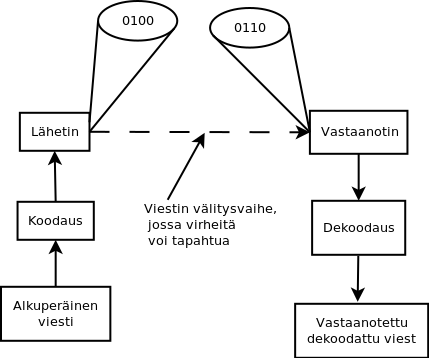
\includegraphics[width=0.6\textwidth]{lahetys}
        \caption{Viestin eteneminen}\label{kuva:lahetys}
    \end{figure}

    Tässä tutkielmassa käsittelemme eri tapoja koodata ja dekoodata viestejä.  Aloitamme hyvin yksinkertaisista esimerkeistä ja siirrymme sitten lähin naapuri dekoodaukseen. Lähin naapuri dekoodauksessa keskitymme ensin minimietäisyyden käyttöön ja sen jälkeen sivuluokkien käyttöön dekoodauksessa. Syvennymme sitten sivuluokkien käyttöön generoijamatriisien ja syndroomien kanssa. 

    Oletetaan, että lukija tuntee joukkojen rakenteet kuten ryhmät, kunnat. Loppu\-osassa tarvitaan myös tietoa sivuluokista, homomorfismista, isomorfismista ja niiden ominaisuuksista.

    %%%%%%%%%%%%%%%%%%%%%%%%%%%%%%%%%%%%%%%%%%%%%%%%%%%%%%%%%%%%%%%%%%%%
    \chapter{Lineaariset binäärikoodit}\label{ch: Lineaariset binäärikoodit}

    Useat kommunikointijärjestelmät käyttävät binäärijärjestelmää. Binäärijärjestelmässä mikä tahansa numero voidaan esittää muodossa, jossa on vain nollia ja ykkösiä.~\cite[s.~266]{GW} Esimerkiksi numero 9 on binäärijärjestelmässä bittijono 1001. Numeroita $n \in \{ 0, 1 \} = \Zset_2$ kutsutaan biteiksi ja merkinnällä $Z_2 = \{ 0, 1 \}$ tarkoitetaan kuntaa, jonka yhteen- ja kertolaskuun ovat modulaarisia.

    Oletetaan, että viesti koostuu $k$ bitistä. Nyt viestiin voidaan lisätä korjausbittejä, joiden avulla voidaan havaita mahdolliset virheet. Muodostetaan siis koodisana, jonka pituus on $n$. Nyt koodisanan viestiosa koostuu $k$ bitistä ja korjausosa $n-k$ bitistä. Tätä pituuden ja korjausbittien suhdetta $R = \frac{k}{n}$ kutsutaan informaatiosuhteeksi~\cite[s.~267]{GW}.
    \begin{esimerkki}\label{esim:3bitsanat}
        Muodostetaan kaikki mahdolliset 3-bittiset sanat. Ne ovat
        \begin{center}
            \begin{tabular}[t]{llll}
                000 & 001 & 011 & 111 \\
                110 & 100 & 101 & 010. \\.
            \end{tabular}
        \end{center}
        Määrittelemme sanoihin neljännen bitin
        $x_4 = (x_1 + x_2 + x_3) \bmod2$. Kaikkien 4 bittisten koodisanojen joukko eli koodi on siis seuraava:
        \[
            C = \{\, x_1x_2x_3x_4 \mid  x_i \in \{0,1\} = \Zset_2, 1 \le i \le 3, x_4 = (x_1 + x_2 + x_3) \bmod2\,\}
        \]
        Huomaamme, että kaikkien bittien summa $x_1 + x_2 + x_3 + x_4$ on aina parillinen, sillä jos kolmen ensimmäisen bitin summa $x_1 + x_2 + x_3$ on parillinen, niin $x_4 = 0$, tai jos summa on pariton, niin $x_4 = 1$.
        Tämän tiedon avulla vastaanottimessa voidaan päätellä, onko välityksessä tapahtunut virhe. Jos sanan kaikkien bittien summa ei ole parillinen, on viesti varmasti väärä. Virhe siis huomataan, mutta ei tiedetä, missä kohtaa se on tapahtunut.[TODO]
    \end{esimerkki}
    \begin{esimerkki}\label{esim:3bitsanatjatko}
        Koodataan sana 101 samaan tapaan kuin
        esimerkissä~\ref{esim:3bitsanat}. Lisätään sitten sanoihin neljäs bitti $x_4 = (x_1 + x_2 + x_3) \bmod2$, joten koodattu sana on 1010. Jatketaan koodausta vielä toistamalla koodattu sana uudelleen eli sanan 101 lopullinen koodattu muoto on 10101010. Oletetaan, että välityksessä tapahtuu yksi virhe. Nyt vastaanottimessa viesti paloittellaan neljän bitin koodisanoihin. Esimerkin~\ref{esim:3bitsanat} mukaan tiedetään, kumpi koodisanoista on väärä, ja täten osataan myös korjata virhe.
    \end{esimerkki}

    \section{Tarvittavien käsitteiden määritelmiä}
    \begin{maaritelma}[vrt. {\cite[s.~491]{PA}}]\label{maar:tarvittavat}
        Olkoon $A$ jokin äärellinen joukko. Kutsumme joukkoa $A$ \emph{aakkostoksi}.

        \begin{enumerate}
            \item Alkiota $u \in  A^n = \underbrace{A \times \cdots \times A}_{
                \text{$n$ kappaletta}}$ kutsutaan \emph{sanaksi}. Sanan $u$ \emph{pituus} on $n$ ja se muodostuu aakkoston $A$ alkioista.
            \item Osajoukkoa $C \subseteq A^n$ kutsutaan \emph{koodiksi}.
            \item Alkiota $u \in C \subseteq A^n$ kutsutaan \emph{koodisanaksi}.
            \item\label{kht:linkoodi} Jos joukko $A$ on kunta, niin $A^n$ on $A$-vektoriavaruus. Jos nyt $C \subseteq A^n$, kutsutaan osajoukkoa $C$ \emph{lineaariseksi koodiksi}. Lisäksi, jos $\dim_A C = k$, kutsutaan osajoukkoa $C$ $(n, k)$-\emph{koodiksi}. Jos $A = \Zset_2$, niin osajoukkoa $C$ kutsutaan \emph{lineaariseksi binäärikoodiksi}.
        \end{enumerate}
    \end{maaritelma}

    \begin{esimerkki}\label{esim:todaliav}
        Esimerkissä~\ref{esim:3bitsanat} esitimme $(4,3)$-koodin
        \[
            C = \{\, x_1x_2x_3x_4 \mid  x_i \in \{0,1\} = \Zset_2, 1 \le i \le 3, x_4 = (x_1 + x_2 + x_3) \bmod2\,\} \subseteq A^4.
        \]
        Silloin $A^4$ on vektoriavaruus, koska $A = \Zset_2$ on kunta. Huomataan, että koodisana $0000 \in C$. 

        Olkoot koodisanat $u \in C$ ja $v \in C$. Nyt koodisanan $u$ kaikkien komponenttien summa on $0 \bmod2$. Täten sama pätee myös koodisanalle $u + v$. Olkoot sitten skalaari $a \in A = \Zset_2$ ja koodisana $u \in C$. Nyt koodisanalle $u$ pätee joko $au = 0$ tai $au = u$.
    \end{esimerkki}

    % \begin{lause}\label{thm: kasautumispisteen ympäristössä}
    %     A on B
    % \end{lause}

    % \begin{proof}
    % Toimii
    % \end{proof}

    \section{Hamming-etäisyys ja -paino}
    \begin{maaritelma}[vrt. {\cite[s.~492]{PA}}]\label{maar:perus}
        Olkoot $u$ ja $v$ sanoja vektoriavaruudesta $A^n$.
        \begin{enumerate}
            \item\label{kht:etaisyys} Sanojen $u$ ja $v$ komponenttien eroavaisuuksien lukumäärää kutsutaan \break{} \emph{Hamming-etäisyydeksi} ja sitä merkitään notaatiolla $d(u,v)$.
            \item\label{kht:paino} Sanan $u$, niiden komponenttien lukumäärää, jotka eroavat nollasta kutsutaan \emph{Hamming-painoksi} ja sitä merkitään notaatiolla
                $\wt(u)$.
            \item Olkoon $r\ge0$ reaaliluku. Nyt joukkoa
                \[
                    S_r(u) = \{\,v \in A^n \mid d(u, v) \le r \,\}
                \]
                kutsutaan sanan $u$ \emph{$r$-palloksi}.
            \item Olkoon $C$ koodi vektoriavaruudessa $A^n$. Koodin $C$ \emph{minimietäisyys} on
                \[
                    d = \min\{\, d(u, w) \mid u, w \in C, u \neq w \,\}.
                \]
        \end{enumerate}
    \end{maaritelma}

    \begin{lause}\label{lause:Hamming}
        Olkoot $u$, $v$ ja $w$ sanoja vektoriavaruudessa $A^n$, missä $A = \Zset_2$. Silloin seuraavat ehdot pätevät:
        \begin{enumerate}
            \item\label{kht:painoetaisyys} $\wt(u) = d(u, 0)$
            \item\label{kht:etaisyyspaino} $d(u, v) = \wt(u - v)$
            \item\label{kht:vaihdannaisuus}$d(u, v) = d(v, u)$
            \item\label{kht:nollaetaisyys} $d(u, v) = 0$, jos $u = v$
            \item\label{kht:kolmioey} $d(u, w) \le d(u, v) + d(v, w)$. \quad (kolmioepäyhtälö)
        \end{enumerate}
    \end{lause}

    \begin{proof}[Todistus \upshape(vrt. {\cite[s.~492]{PA}})]\label{tod: Hamming}
        Lauseen~\ref{lause:Hamming} kohta~\ref{kht:painoetaisyys} seuraa suoraan määritelmän~\ref{maar:perus} kohdista~\ref{kht:etaisyys} ja~\ref{kht:paino}.

        Kohdassa~\ref{kht:etaisyyspaino} sanan $u - v$ komponentti kohdassa $i$ on 1, jos sanat $u$ ja $v$ eroavat komponentissa~$i$. Nyt määritelmän perusteella saadaan $\wt(u - v) = d(u, v)$.

        Kohta~\ref{kht:vaihdannaisuus} seuraa suoraan määritelmän~\ref{maar:perus} kohdasta~\ref{kht:etaisyys}.

        Kohdassa~\ref{kht:nollaetaisyys} sanojen $u$ ja $v$ etäisyys $d(u, v) = 0$, jos sanojen $u$ ja $v$ kaikki komponentit kohdassa $i$ ovat samoja, kun $1 \le i \le n$.

        Kohdan~\ref{kht:kolmioey} todistus on hieman pidempi kuin muut. Olkoot $x = u - v$ ja $y = v - w$. Nyt lauseen~\ref{lause:Hamming} kohdan~\ref{kht:etaisyyspaino} nojalla epäyhtälön vasemmasta puolesta saadaan
        \[
            d(u,w) = \wt(u - w) = \wt(x + y).
        \]
        Samoin oikeasta puolesta saadaan
        \begin{gather*}
            d(u,v) = \wt(u - v) = \wt(x)\text{~ja} \\
            d(v,w) = \wt(v - w) = \wt(y).
        \end{gather*}
        Todistettava epäyhtälö on siis
        \[
            \wt(x + y) \le \wt(x) + \wt(y).
        \]
        Olkoot $x_i$ ja $y_i$ sanojen $x$ ja $y$ kohdassa $i$ olevia komponentteja. Olkoon myös sana $z = x + y$ ja sen kohdassa $i$ oleva komponentti $z_i$. Huomaamme, että
        \[
            \wt(x + y) = \sum_{i = 1}^n z_i \qquad \wt(x) = \sum_{i =1}^n x_i \qquad \wt(y) = \sum_{i = 1}^n y_i.
        \]
        Riittää siis todistaa, että $z_i \le x_i + y_i$ kaikilla $1 \le i \le n$. Tämä seuraa kuitenkin suoraan siitä, että $z_i = x_i + y_i \bmod 2$.
    \end{proof}

    \begin{esimerkki}\label{esim:minetaisyys}
        Tarkastellaan sitten yhtä etäisyyden käyttömahdollisuutta välityksessä. Oletetaan, että viestin välityksessä tapahtuu yksi virhe. Silloin vastaanotetun koodisanan ja oikean koodisanan etäisyys on 1. Määritellään seuraavaksi koodi $C$, jonka minimietäisyys on $d = 3$.

        Esimerkissä~\ref{esim:3bitsanat} listasimme kaikki aakkoston $A^3$ sanat, missä $A = \Zset_2$. Koodataan nämä sanat lisäämällä kolme uutta komponenttia. Määritellään koodi $C \subseteq A^6$ seuraavasti:
        \begin{gather*}
            x_1x_2x_3x_4x_5x_6 \in C, \text{ jos} \\
            x_4 = x_1 + x_2 \\
            x_5 = x_1 + x_3 \\
            x_6 = x_2 + x_3.
        \end{gather*}
        % TODO Tähän se aliavaruus testi
        Listataan sitten uudelleen kaikki vektoriavaruuden $A^3$ sanat ja niiden koodisanat koodissa $C \subseteq A^6$. Saadaan taulukko
        \begin{center}
            \begin{tabular}[t]{ll}
                sana & koodisana \\ \midrule
                000 & 000000\\
                001 & 001011\\
                011 & 011110\\
                111 & 111000\\
                110 & 110011\\
                100 & 100110\\
                101 & 101101\\
                010 & 010101\\
            \end{tabular}
        \end{center}
        
        Tarkastellaan seuraavaksi sanojen etäisyyttä toisistaan. Valitaan ensin sanat, joiden etäisyys toisistaan on 1. Valitaan esimerkiksi sanat $110$ ja $100$. Niiden vastaavat koodisanat ovat $u = 110011 \in C$ ja $v = 100110 \in C$. Nyt alkuperäiset sanat eroavat vain yhdessä komponentissa, mutta niiden koodisanat eroavat kolmessa komponentissa eli $d(u,v) = 3$. Yleisesti, jos kaksi sanaa eroavat vain komponentissa $i$, komponentti $i$ esiintyy kahdessa yhtälössä, jotka määrittelimme koodin $C$ tarkastuskomponenteille
        $x_4$, $x_5$ ja $x_6$. Koodisanojen etäisyys on siis vähintään 3.

        Tarkastellaan sitten sanoja, joiden etäisyys on 2. Valitaan sanat $110$ ja $101$. Olkoot niiden vastaavat koodisanat $u = 110011 \in C$ ja $v = 101101 \in C$, joiden etäisyys on $d(u, v) = 4$. Yleisesti jos sanat eroavat komponenteissa $i$ ja $j$, kahdessa yhtälöistä, jotka määrittelimme komponenteille $x_4x_5x_6$, esiintyy komponentti $i$, mutta ei komponenttia $j$ tai komponentti $j$, mutta ei komponenttia $i$. [ TODO CHECK THIS]

        Tarkastellaan sitten sanoja, joiden etäisyys toisistaan on 3. Jos jo sanojen etäisyys on 3, on koodisanojenkin etäisyys vähintään kolme, sillä sanat sisältyvät sellaisenaan koodisanaan. Täten olemme osoittaneet, että minimietäisyys tässä tapauksessa on $d = 3$.

        Oletetaan, että lähetettävä sana on 001 ja sen vastaava koodisana $u = 011110 \in C$.
        Alussa oletettiin, että lähetyksessä tapahtuu yksi virhe. Kutsutaan tätä vastaanotettua koodisanaa koodisanaksi $v$. Koska koodin $C$ minimietäisyys on $d = 3$, on lähetty koodisana $u$ ainoa, jonka etäisyys vastaanotetusta koodisanasta $v$ on $d(u,v) = 1$.
    \end{esimerkki}

    \begin{maaritelma}[vrt. {\cite[s.~494]{PA}}]\label{maar:nkkoodi}
        Olkoot $C$ $(n, k)$-koodi ja $u = x_1x_2x_3\dots x_k \dots x_n \in C$ sen eräs koodisana. Nyt koodisanan $u$ ensimmäiset $k$ komponenttia muodostavat alkuperäisen viestin ja viimeisiä $n-k$ komponenttia kutsutaan pariteetintarkastuskomponenteiksi.
    \end{maaritelma}

    \chapter{Virheenkorjaaminen}
    \section{Minimietäisyys}

    \begin{lause}\label{lause:nncorrection}
        Olkoon koodi $C \subseteq A^n$ ja sen minimietäisyys $d$. Jos käytämme lähin naapuri dekoodausta, niin kaikille $t \in \Nset$ pätevät seuraavat ehdot:
        \begin{enumerate}
            \item\label{kht:vtunnistus} Koodi $C$ voi tunnistaa ainakin $t$ kappaletta virheitä, jos $t + 1 \le d$.
            \item\label{kht:vkorjaus} Koodi $C$ voi korjata ainakin $t$ kappaletta virheitä, jos $2t + 1 \le d$.
        \end{enumerate}
    \end{lause}

    \begin{proof}[Todistus \upshape(vrt. {\cite[s.~494]{PA}})]\label{tod:nncorrection}
        Aloitetaan lauseen~\ref{lause:nncorrection} kohdasta~\ref{kht:vtunnistus}. Olkoot koodi $C \subseteq A^n$ ja sen minimietäisyys $d$. Valitaan sitten koodisana $u \in C$. Nyt pallo $S_t(u)$ sisältää kaikki mahdolliset vastaanotetut sanat, jos lähetetty koodisana oli $u$ ja välityksessä tapahtui enintään $t$ virhettä. Jos koodin $C$ minimietäisyys $d < t$, niin pallo $S_t(u)$ sisältää vain koodisanan $u$. Täten jos virheitä tapahtuu enintään $t$ kappaletta, niin vastaanotettu sana $w$ ei ole koodisana. Näin voimme tunnistaa, jos virheitä on tapahtunut enintään $t$ kappaletta.

        Kohdassa~\ref{kht:vkorjaus} aloitetaan samalla tavalla. Olkoot koodi $C \subseteq A^n$ ja sen minimietäisyys $d$. Valitaan sitten kaksi koodisanaa $u, v \in C$ siten, että $u \neq v$. Jos minimietäisyydelle pätee $2t < d$, niin vastaanotettu sana $w$ ei voi sisältyä molempiin palloihin $S_t(u)$ ja $S_t(v)$. Tämä voidaan osoittaa olettamalla ensin, että sana $w$ kuuluu molempiin palloihin. Nyt kolmioepäyhtälöstä saadaan
        \[
            d(u,v) \le d(u,w) + d(w, v) \le t + t < d,
        \]
        joka on ristiriidassa minimietäisyyden määritelmän kanssa. Täten vastaanotettu sana $w$ voidaan aina korjata lähimpään koodisanaan.
    \end{proof}

    Rajoitutaan loppuosassa binäärikoodeihin eli $A = \Zset_2$.
    \begin{esimerkki}
        Tarkastellaan seuraavaksi esimerkin~\ref{esim:minetaisyys} $(6,3)$-koodia $C$. Esimerkissä totesimme, että koodin $C$ minimietäisyys $d = 3$. Nyt siis jos $t = 1$, koodi $C$ osaa korjata lähetyksessä tapahtuneet virheet. Jos $t = 2$, koodi $C$ tunnistaa virheet, mutta ei osaa korjata niitä.

        Oletetaan, että lähetetty koodisana oli $111000 = u \in C$ ja vastaanotettu sana $011001= w \in C$. Koska sana $w$ ei ole koodisana, voimme tunnistaa, että lähetyksessä on tapahtunut virheitä. Nyt kuitenkin $d(u,w) = 2$ ja $d(u,v) = 2$, missä koodisana $v = 001011$. Emme voi siis tietää kumpi koodisanoista oli alun perin lähetetty.
    \end{esimerkki}

    \section{Sivuluokkadekoodaus}
    \begin{lause}\label{lause:Hammingraja}
        Olkoon $C$ $(n, k)$-koodi, jonka minimietäisyys on $d \ge 2t +1$. Nyt siis koodi $C$ osaa korjata $t$ virhettä käyttämällä lähin naapuri dekoodausta. Hamming-rajaksi kutsutaan seuraavaa epäyhtälöä:
        \[
            2^k = \abs{C} \le \frac{2^n}{\binom{n}{0}+\binom{n}{1}+\binom{n}{2}+\cdots+\binom{n}{t}},
        \]
        \[
            \text{missä} \quad \binom{n}{b} = \frac{n!}{b!(n-b)!}
        \]
        on binomikerroin ja $\abs{C}$ on koodin $C$ koodisanojen lukumäärä.
    \end{lause}

    \begin{proof}[Todistus \upshape(vrt. {\cite[s.495]{PA}})]\label{tod:Hammingrajoitus}
        Olkoon koodin $C \subseteq \Zset_2^n$ dimensio $\dim_{\Zset_2}(C) = k$. Täten koodin $C$ koodisanojen lukumäärä on $\abs{C} = 2^k$. Olkoon sitten koodisana $u \in C$. Nyt koodisana $w \in S_t(u)$, jos sanojen etäisyys $d(u,w) \le t$. Koodisanassa $u$ on $n$ komponenttia, joten binomikertoimesta $n! / b!(n-b)\!$ saadaan sanat, jotka eroavat sanasta $u$ $b$ komponentissa. Nyt pallon $S_t(u)$ sanojen lukumäärä on siis
        \[
            \abs{S_t(u)} = \binom{n}{0} + \binom{n}{1} +\binom{n}{2} +  \cdots + \binom{n}{t}.
        \]
        Koska $2t + 1 \le d$, niin ei ole olemassa alkiota $a \in S_t(u)$ ja $a \in S_t(v)$. Toisin sanoen palloissa ei ole yhteisiä alkioita eli ne ovat erilliset. Nyt siis alkioita kaikissa palloissa on yhteensä
        \[
            \sum_{u \in C}\abs{S_t(u)} = \abs{S_t(u)}\abs{C}.
        \]
        Kuitenkin vektoriavaruudessa $A^n$ alkioita on yhteensä $2^n$ kappaletta, koska $A = \Zset_2$.
        Tästä seuraa seuraava epäyhtälö:
        \begin{align*}
            \abs{S_t(u)}\abs{C} &\le 2^n \\
            \abs{C} &\le \frac{2^n}{\abs{S_t(u)}} \\
            \abs{C} &\le \frac{2^n}{\binom{n}{0} + \binom{n}{1} +\binom{n}{2} +  \cdots + \binom{n}{t}}.
        \end{align*}
    \end{proof}

    Olkoot $C$ $(n,k)$-koodi ja joukko $A = \Zset_2$. Nyt vektoriavaruus $A^n$ on Abelin ryhmä yhteenlaskun suhteen, sillä vektoriavaruuden aksioomiin sisältyy kaikki Abelin ryhmän aksioomat. Abelin ryhmän $A^n$ alkioiden lukumäärä on $2^n$. Nyt koodi $C$ on Abelin ryhmän $A^n$ aliryhmä yhteenlaskun suhteen ja se sisältää $2^k$ koodisanaa. Koodilla $C$ on nyt $\frac{\abs{A^n}}{\abs{C}} = \frac{2^n}{2^k} = 2^{n-k}$ sivuluokkaa vektoriavaruudessa $A^n$.

    Seuraavaksi esittelemme sivuluokkadekoodauksen koodin $C$ sivuluokkien avulla. Valitaan ensin jokaisesta sivuluokasta sana $u_i \in C$ siten, että sanalla $u$ on pienin paino. Nyt jokainen sivuluokka on seuraavaa muotoa:
    \[
        u_1 + C, u_2 + C, \dots, u_N + C,
    \]
    \[
        \text{missä } N = 2^{n-k}.
    \]
     Valittuja sanoja $u_i$ kutsutaan \emph{sivuluokan johtajiksi}. Jos vastaanotetaan sana $w$, niin sanan $w$ täytyy kuulua johonkin sivuluokkaan. Nyt siis sana $w \in u_i + C$, joten se voidaan dekoodata takaisin koodisanaksi vähentämällä siitä sana $u_i$. Dekoodattu sana on siis $w - u_i \in C$. Tämä dekoodaus voidaan helposti toteuttaa muodostamalla koodille $C$ \emph{standardikaavio}.

    \begin{esimerkki}\label{esim:stdmatrix}
        Olkoon $(4,2)$-koodi $C = \{\,0000,\, 0110,\, 1011\,,1101\,\}$. Muodostetaan koodille $C$ standardikaavio. Saadaan
        \begin{center}
            \begin{tabular}{llll}
                0000 & 0110 & 1011 & 1101 \\ \midrule
                1000 & 1110 & 0011 & 0101 \\
                0100 & 0010 & 1111 & 1001 \\
                0001 & 0111 & 1010 & 1100
            \end{tabular}
        \end{center}
        Ensimmäisessä rivissä on kaikki koodin $C$ koodisanat ja ensimmäisessä sarakkeessa kaikki sivuluokkien johtajat. Muut rivit on muodostettu valitsemalla vähiten painava sana $u$ vektoriavaruudesta $A^4 = \Zset_2^4$ ja sijoittamalla se rivin vasempaan reunaan. Sitten loput sanat ovat saatu laskemalla sana $u$ yhteen koodin $C$ koodisanojen kanssa.

        Oletetaan, että vastaanotetaan sana 0010. Nyt sana 0010 esiintyy taulukon kolmannessa rivissä ja toisessa sarakkeessa. Taulukon kolmannen rivin vasemmasta reunasta nähdään sen sivuluokan johtaja 0100, joten vastaanotetun sanan sivuluokka on $0100 + C$. Täten vastaanotettu sana 0010 voidaan dekoodata $0010 - 0100 = 0110$.
    \end{esimerkki}

    \begin{lause}\label{lause:nnstdarr}
        Sivuluokka dekoodaus on lähin naapuri dekoodausta.
    \end{lause}

    \begin{proof}[Todistus \upshape(vrt. {\cite[s.~496]{PA}})]\label{tod:nnstdarr}
        Olkoot $C$ $(n,k)$-koodi ja vastaanotettu sana $w \in u + C$, missä sana $u$ on sivuluokan johtaja. Nyt sana $w$ voidaan dekoodata $w - u = v \in C$. Haluamme osoittaa, että epäyhtälö $d(w,v) \le d(w, y)$ pätee jokaiselle $y \in C$. Käytetään ensin lauseen~\ref{lause:Hamming} kohtaa~\ref{kht:etaisyyspaino}, josta saadaan
        \[
            d(w,v) = \wt(w-v) = \wt(u). %\le \wt(w-y) = d(w,y).
        \]
        Koska sivuluokka voidaan merkitä sen minkä tahansa alkion avulla, jokaiselle $y \in C$ pätee $w - y \in w + C = u + C$. Tästä saadaan epäyhtälö
        \[\wt(u) \le \wt(w-y) = d(w,y).\]
    \end{proof}

    \chapter{Generoijamatriisit}
    Lineaariset binäärikoodit eli $(n,k)$-koodit koostuvat $n$ bitin pituisista koodisanoista. Näitä koodisanoja on yhteensä $2^k$ kappaletta. Koodin kaikkien koodisanojen listaamisesta tulee nopeasti erittäin työlästä ja epäkäytännöllistä. Voimme kuitenkin tiivistää kaiken tarvittavan tiedon $k \times n$-matriisiin.

    \begin{esimerkki}\label{esim:genmatrix}
        Valitaan seuraava $3 \times 6$-matriisi:
        \[
            G=
            \begin{bbmatrix}
                1 & 0 & 0 & 1 & 1 & 0\\
                0 & 1 & 0 & 1 & 0 & 1\\
                0 & 0 & 1 & 0 & 1 & 1
            \end{bbmatrix}.
        \]
        Nyt jokainen sana $x_1x_2x_3$ voidaan kirjoittaa $1 \times 3$-matriisina. Kun alkuperäinen koodattava sana kerrotaan matriisilla $G$, saadaan koodin $C$ koodisana. Saamme koodisanaksi
        \[
           \begin{bmatrix}
               x_1 & x_2 & x_3
            \end{bmatrix}G =
            \begin{bmatrix}
                x_1 & x_2 & x_3 & x_4 & x_5 & x_6
            \end{bmatrix},
        \]
        missä $x_4 = x_1 + x_2$, $x_5 = x_1 + x_3 $ ja $x_6 = x_2 + x_3$. Koodi $C$ on siis määritelty samoin kuin esimerkissä~\ref{esim:minetaisyys}. Esimerkiksi, jos halutaan lähettää sana 011, saamme koodisanaksi
        \[
           \begin{bmatrix}
               0 & 1 & 1
            \end{bmatrix}
            G =
            \begin{bmatrix}
                0 & 1 & 1 & 1 & 1 & 0
            \end{bmatrix},
        \]
        joka näkyy myös esimerkin~\ref{esim:minetaisyys} taulukosta. Täten koodi
        \[
            C = \{\,wG \mid w \in A^k\,\}
        \]
        ja matriisi $G$ sisältää kaiken tarvittavan tiedon sanojen koodaamiseen.
    \end{esimerkki}

    \begin{maaritelma}[vrt. {\cite[s.~497]{PA}}]\label{maar:generoija}
        Olkoon $G$ $k \times n$-generoijamatriisi. Nyt \emph{generoijamatriisi} on
        \[
            G = 
            \begin{bmatrix}
                I_k & B 
            \end{bmatrix},
        \]
        missä $I_k$ on $k \times k$-identiteettimatriisi ja $B$ on $k \times (n-k)$-binäärimatriisi. 
    \end{maaritelma}

    \begin{esimerkki}
        Esimerkiksi esimerkin~\ref{esim:stdmatrix} generoijamatriisi on
        \[
            C =
            \begin{bbmatrix}
                1 & 0 & 1 & 1\\
                0 & 1 & 1 & 0\\
            \end{bbmatrix},
        \]
        \[
            \quad \text{missä }I_k = 
            \begin{bmatrix}
                1 & 0 \\
                0 & 1
            \end{bmatrix}\text{ ja }
            B =
            \begin{bmatrix}
                1 & 1 \\
                1 & 0
            \end{bmatrix}.
        \]
    \end{esimerkki}

    \section{Systemaattiset koodit}

    \begin{maaritelma}[vrt. {\cite[s.~498]{PA}}]\label{maar:systemaattinen}
        Kutsumme $(n, k)$-koodia \emph{systemaattiseksi koodiksi}, jos sana $u \in A^k$ muodostaa täsmälleen yhden koodisanan $v \in C$ ensimmäiset $k$ komponenttia. Toisin sanoen koodissa $C$ on olemassa vain yksi koodisana  siten, että $u_i = v_i$, kaikilla $i \in [1,k]$.
    \end{maaritelma}

    \begin{apulause}\label{apu:isomorfia}
        Olkoot $G$ ja $G'$ ryhmiä ja funktio $\phi: G \rightarrow G'$ homomorfismi. Olkoon myös ydin $K = \ker(\phi) = \{\,g \in G \mid \phi(g) = 0_{G'}\,\}$, missä $0_{G'}$ on ryhmän $G'$ neutraalialkio. Nyt pätee isomorfia
        \[
            G/K \cong \phi(G).
        \]
    \end{apulause}

    \begin{proof}[Todistus \upshape(vrt. {\cite[s.~97]{PA}})]\label{tod:isomorfia}
        Olkoon funktio $\chi: G/K \rightarrow \phi(G)$. Nyt joukon $G/K$ mikä tahansa alkio on sivuluokka $gK$, jollain $g \in G$. Jokainen alkio $y \in \phi(G)$ on muotoa $\phi(g)$, jollain $g \in G$. Määrittelemme nyt funktion $\chi$ siten, että $\chi(gK) = \phi(g)$. Tarkastellaan ensin funktion $\chi$ on yksikäsitteisyyttä. Toisin sanoen, jos valitaan kaksi samaa alkiota $g_1K = g_2K$ ja siitä seuraa, että $\phi(g_1) = \phi(g_2)$, niin on funktio $\chi$ yksikäsitteinen.
        Oletetaan ensin, että $g_1K = g_2K$. Nyt, kun alkiot ovat samat niin $g_1g_2^{-1} \in K$, jolloin saamme
        \[
            \phi(g_1g_2^{-1}) = 0_{G'}.
        \]
        Koska funktio $\phi$ on ryhmähomomorfismi voimme kirjoittaa ylemmän yhtälön:
        \begin{align*}
            \phi(g_1){\phi(g_2)}^{-1} &= 0_{G'} \\
            \phi(g_1) &= \phi(g_2).
        \end{align*}
        Nyt siis funktio $\chi$ on yksikäsitteinen.

        Olkoon $g_1K$ ja $g_2K$ kaksi alkiota joukosta $G/K$. Nyt saamme
        \[
            \chi(g_1Kg_2K) = \chi(g_1g_2K) = \phi(g_1g_2) = \phi(g_1)\phi(g_2) = \chi(g_1K)\chi(g_2K),
        \]
        joten funktio $\chi$ on ryhmähomomorfismi.

        Olkoot $g_1K$ ja $g_2K$ kaksi alkiota joukosta $G/K$, joille pätee $\chi(g_1K) = \chi(g_2K)$.
        Nyt $\phi(g_1) = \phi(g_2)$, joten $\phi(g_1)\phi^{-1}(g_2) = 0_{G'}$. Saamme siis $\phi(g_1g_2^{-1}) = 0_{G'}$ eli $g_1g_2^{-1} \in K$, joten $g_1K = g_2K$. Olemme nyt osoittaneet, että funktio $\chi$ on injektio.

        Olkoon $y$ jokin joukon $\phi(G)$ alkio. Nyt alkio $y = \phi(x)$, jollakin alkiolla $x \in G$. Funktion $\chi$ määritelmän perusteella saamme 
        \begin{align*}
            \chi(xK) &= \phi(x) \\
            \chi(xK) &= y,
        \end{align*}
        joten funktio $\chi$ on surjektio.

        Täten $\chi: G/K \rightarrow \phi(G)$ on isomorfismi ja
        \begin{align*}
            G/K &\cong K \\
            G/\ker(\phi) &\cong K.
        \end{align*}
    \end{proof} 

    \begin{lause}\label{lause:systemaattinen}
        \mbox{}
        \begin{enumerate}
            \item\label{kht:sysmatr} Olkoon $G$ $k \times n$-matriisi. Nyt koodi $C = \{\, vG \mid v \in A^k\,\} \subseteq A^n$ on systemaattinen $(n, k)$-koodi.
            \item\label{kht:sysgenmatr} Olkoon $C \subseteq A^n$ systemaattinen $(n, k)$-koodi. Nyt on olemassa $k \times n$-generoija\-matriisi siten, että $C = \{\, vG \mid v \in A^k\,\}$.
        \end{enumerate}
    \end{lause}

    \begin{proof}[Todistus \upshape(vrt. {\cite[s.~498]{PA}})]\label{tod:systemaattinen}
        % TODO tarviiko todistaa että ne on ryhmiä? EI KAI. On tässä vitusti vaikeempaaki paskaa
        Aloitetaan lauseen~\ref{lause:systemaattinen} kohdasta~\ref{kht:sysmatr}. Olkoot matriisi $G$ $k \times n$-generoijamatriisi ja koodi $C = \{\, vG \mid v \in A^k\,\}$. Koska kaikki vektoriavaruudet $A^r$ ovat Abelin ryhmiä yhteenlaskun suhteen, kun $r \ge 0$, voidaan määritellä funktio $\phi: A^k \rightarrow A^n$ siten, että $\phi(v) = Gv \in A^n$. Nyt tämä on ryhmähomomorfismi, sillä jokaiselle $u, v \in A^k$ pätee
        \[
            \phi(v + u) = (v + u)G = vG + uG = \phi(v) + \phi(u).
        \]

        Nyt siis koodi $C$ on funktion $\phi$ kuvajoukko $\im(\phi)$. Määritelmän~\ref{maar:generoija} perusteella
        $G = 
        \begin{bmatrix}
            I_k & B
        \end{bmatrix}$, joten
        \[
            \phi(v) =
            \begin{bmatrix}
                v & vB
            \end{bmatrix}
            =
            \begin{bmatrix}
                u & uB
            \end{bmatrix}
            = \phi(u),
        \]
        jos ja vain jos $u = v$. Täten sana $u \in A^k$ kuvautuu vain yhtenä koodisanana koodissa $C$ ja siis funktio $\phi$ on injektio. Apulauseen~\ref{apu:isomorfia} perusteella vektoriavaruus $A^k \cong C$ ja koodi $C$ on ryhmän $A^n$ aliryhmä. Täten määritelmän~\ref{maar:tarvittavat} kohdan~\ref{kht:linkoodi} perusteella $C$ on $(n, k)$-koodi. Koodi $C$ on myös systemaattinen, sillä funktio $\phi$ on yksikäsitteinen.

        Tarkastellaan sitten kohtaa~\ref{kht:sysgenmatr}. Olkoon koodi $C$ systemaattinen $(n, k)$-koodi. Muodostamme sitten generoijamatriisin $G$. Olkoon $\{e_i\}$ luonnollinen kanta vektoriavaruudelle $A^k$. Koska koodi $C$ on systemaattinen, jokaiselle $1 \le i \le k$ on olemassa eri koodisana $c_i \in C$. Nyt siis koodisana 
        $c_i = 
        \begin{bmatrix}
            e_i & d_i
        \end{bmatrix}
        $, missä koodisanan $c_i$ ensimmäiset $k$ komponenttia ovat vektori $e_i$ ja $d_i$ on jokin vektori vektoriavaruudesta $A^{n-k}$. Olkoon nyt $B$ $k \times (n-k)$-matriisi, missä on sanat $d_i$ riveinä. Olkoon myös generoijamatriisi 
        $G =  
        \begin{bmatrix}
            I_k & B
        \end{bmatrix}$.
        Haluamme nyt osoittaa, että koodi $C = \{\,vG \mid v \in A^k\,\}$. Koska 
        \[
            e_i B  =
            \begin{bmatrix}
                0 & \cdots & 0 & 1 & 0 & \cdots & 0
            \end{bmatrix}
            \begin{bbmatrix}
                d_1 \\
                \vdots \\
                d_i \\
                \vdots \\
                d_k
            \end{bbmatrix}
            =
            \begin{bmatrix}
                d_i
            \end{bmatrix}
        \]
        eli $e_i B$ on matriisin $B$ rivi kohdassa $i$, kun $1 \le i \le k$.
        Nyt saamme kaikille $1 \le i \le k$
        \[
            e_i G = e_i
            \begin{bmatrix}
                I_k & B
            \end{bmatrix}
            =
            \begin{bmatrix}
                e_i & e_i B
            \end{bmatrix}
            =
            \begin{bmatrix}
                e_i & d_i
            \end{bmatrix}
            =
            c_i \in C.
        \]
        Nyt koska $e_i$ oli luonnollinen kanta vektoriavaruudelle $A^k$, saamme
        \[
            \{\,vG \mid v \in A^k\,\} \subseteq C.
        \]
        Olkoon $c \in C$, missä 
        $c = 
        \begin{bmatrix}
            u & w
        \end{bmatrix}$, $u \in A^k
        $ ja $w \in A^{n-k}$. Nyt saamme
        \[
            uG = u
            \begin{bmatrix}
                I_k & B  
            \end{bmatrix}
            = 
            \begin{bmatrix}
                u & uB
            \end{bmatrix}
            = 
            \begin{bmatrix}
                u & w'  
            \end{bmatrix}
            \in C, \quad \text{missä } w' \in A^{n-k}.
        \]
        Mutta koska koodi $C$ on systemaattinen, saamme määritelmän~\ref{maar:systemaattinen} perusteella
        \[
            \begin{bmatrix}
                u & w'  
            \end{bmatrix}
            =
            \begin{bmatrix}
                u & w  
            \end{bmatrix}
            = c = uG.
        \]
        Täten olemme osoittaneet, että
        \[
            C \subseteq \{\,vG \mid v \in A^k\,\}.
        \]
        Olemme osoittaneet nyt, että koodi $C = \{\,vG \mid v \in A^k\,\}$.
    \end{proof} 

    \chapter{Syndroomat}
    Generoijamatriisit ovat käteviä sanoja koodatessa. Tarvitsemme vielä tavan dekoodata vastaanotetut sanat helposti. Tarkastellaan seuraavaksi syndrooma tapaa tähän tarkoitukseen.
    \begin{maaritelma}[{\cite[s.~499]{PA}}]\label{maar:parcheckmatrix}
        Olkoon $C$ systemaattinen $(n, k)$-koodi, jolla on generoijamatriisi 
        $G = 
        \begin{bmatrix}
            I_k & B  
        \end{bmatrix}
        $. Nyt $n \times (n-k)$-matriisia
        \[
            H =
            \begin{bbmatrix}
                B \\
                I_{n-k}
            \end{bbmatrix}
        \]
        kutsutaan \emph{pariteetintarkastusmatriisiksi}. Olkoon sana $w \in A^n$. Nyt sanan $w$ \emph{syndrooma} on $wH \in A^{n-k}$.
    \end{maaritelma}

    \begin{esimerkki}\label{esim:parcheckmatrix}
        Esimerkissä~\ref{esim:stdmatrix} pariteetintarkastusmatriisi oli
        \[
            H = 
            \begin{bbmatrix}
                1 & 1 \\
                1 & 0 \\
                1 & 0 \\
                0 & 1
            \end{bbmatrix}.
        \]
    \end{esimerkki}

    \begin{lause}\label{lause:sanojensyndroomat}
        Olkoon $C$ systemaattinen $(n, k)$-koodi, jolla on generoijamatriisi $G$ ja pariteetintarkastusmatriisi $H$. Olkoon myös sana $v \in A^n$. Nyt sanan $v$ syndrooma $vH = 0 \in A^{n-k}$, jos ja vain jos $v \in C$.
    \end{lause}

    \begin{proof}[Todistus \upshape(vrt. {\cite[s.~499]{PA}})]\label{tod:sanojensyndroomat}
        Kuten lauseen~\ref{lause:systemaattinen} todistuksessa, käytetään tässäkin hyväksi tietoa, että kunnasta muodostettu vektoriavaruus on Abelin ryhmä yhteenlaskun suhteen. Määritellään funktio $\phi:A^n \rightarrow A^{n-k}$ siten, että $\phi(v) = vH$ jokaiselle $v \in A^n$. Nyt jokaiselle $u, v \in A^n$ pätee
        \[
            \phi(u + v) = (v + u)H = uH + vH = \phi(u) + \phi(v)
        \]
        Täten funktio $\phi$ on ryhmähomomorfismi. Funktio $\phi$ on myös surjektio, sillä olkoot $w \in A^{n-k}$ ja vektori 
        $v =
        \begin{bmatrix}
            0 & w  
        \end{bmatrix}
        \in A^n$. Nyt vektorin $v$ ensimmäiset $k$ komponenttia ovat nollia ja loput $n-k$ komponenttia vektorin $w$ komponentteja. Nyt siis
        \[
            \phi(v) = vH =
            \begin{bmatrix}
                0 & w 
            \end{bmatrix}
            \begin{bbmatrix}
               B \\
               I_{n-k}
            \end{bbmatrix}
            = 0B + wI_{n-k} = w.
        \]
    Täten löysimme jokaiselle $w \in A^{n-k}$ vektorin $v \in A^n$ siten, että $\phi(v) = w$. Nyt siis funktio $\phi$ on surjektio.
    Apulauseella~\ref{apu:isomorfia} saamme
    \[
        A^n/\ker(\phi) \cong A^{n-k}.
    \]
    Täten $\abs{\ker(\phi)} = \abs{A}^k = \abs{C}$. Osoitetaan vielä, että $C \subseteq \ker(\phi)$. Olkoon koodisana $v \in C$. Koska $C$ on systemaattinen koodi, $v = wG$, jollekin sanalle $w \in A^k$. Täten $\phi(v) = vH = wGH = 0$, sillä
    \[
        GH =
        \begin{bmatrix}
            I_k & B
        \end{bmatrix}
        \begin{bbmatrix}
            B \\
            I_{n-k}
        \end{bbmatrix}
        = B + B = 0
    \]
    Nyt siis koodisana $v \in \ker(\phi)$ ja koodi $C \subseteq \ker(\phi)$.
    Koska $\abs{\ker(\phi)} = \abs{C}$, niin on oltava $C = \ker(\phi)$.
    \end{proof} 

    \begin{lause}\label{lause:sivuluokkiensyndroomat}
        Olkoon $C$ systemaattinen $(n, k)$-koodi, jolla on generoijamatriisi $G$ ja pariteetintarkastusmatriisi $H$. Nyt sanat $u$ ja $v$ ovat samassa sivuluokassa, jos ja vain jos sanoilla $u$ ja $v$ on sama syndrooma.
    \end{lause}

    \begin{proof}[Todistus \upshape(vrt. {\cite[s.~500]{PA}})]\label{tod:sivuluokkiensyndroomat}
        Olkoot sanat $u, v \in A^n$. Aloitetaan olettamalla, että sivuluokat ovat samat. Silloin
        \[
            u + C = v + C \quad \text{, jos ja vain jos} \quad u - v \in C.
        \]
        Nyt lauseen~\ref{lause:sanojensyndroomat} perusteella saamme, että $u - v \in C$, jos ja vain jos
        \begin{align*}
            (u - v)H &= 0 \\
            uH &= vH.
        \end{align*}
        Täten sanojen $u$ ja $v$ syndroomat ovat samat.
    \end{proof} 

    \begin{esimerkki}
        Olkoon $C$ esimerkin~\ref{esim:stdmatrix} $(4,2)$-koodi, jonka pariteetintarkastusmatriisi H esitettiin esimerkissä~\ref{esim:parcheckmatrix}. Esitetään seuraavaksi jokaisen sivuluokan syndroomat. Ensimmäisellä rivillä on sivuluokan johtajat ja toisella niiden syndroomat.
        \begin{center}
            \begin{tabular}{llllll}
                v && 0000 & 1000 & 0100 & 0001 \\
                vH  &&  00 & 11 & 10 & 01
            \end{tabular}
        \end{center}
        Oletetaan sitten, että vastaanotetaan sana $u = 0111$. Nyt sanan $u$ syndrooma on $uH = 01$, joten $u$ on sivuluokassa, jonka johtaja on sana $v =0001$. Dekoodaamme sanan $u$ siis $u - v = 0110 \in C$.
        
        Osaamme nyt dekoodata viestejä syndroomien avulla. Tämä on paljon kätevämpää kuin muodostaa standardikaavio, kuten esimerkissä~\ref{esim:stdmatrix}.
    \end{esimerkki}

    \begin{thebibliography}{9}
        % LaTeX ei oletusarvoisesti lisää lähdeluettelon otsikkoa sisällysluetteloon, joten se on tehtävä tässä erikseen:
        \addcontentsline{toc}{chapter}{\bibname}

        % \bibitem{Mathman}
        % Mathman, Z. \emph{An elementary course in mathematical analysis}.
        % New York: Birch and Star, 1990.
        \bibitem{GW}
        Gilbert, W. J. \& Nicholson, W. K.
        \emph{Modern Algebra with Applications. 2nd edition}.
        John Wiley \& Sons, 2004.

        \bibitem{PA}
        Papantonopoulou, A.
        \emph{Algebra Pure \& Applied}.
        Prentice-Hall, 2002.


\end{thebibliography}

\end{document}
